\documentclass{llncs}

\usepackage{url}
\usepackage{graphicx}
\usepackage{listings}
\usepackage{verbatim}
\usepackage[lined,linesnumbered,algochapter]{algorithm2e}
\usepackage{tikz}
\usetikzlibrary{arrows,automata}
\usepackage{xspace}
\usepackage{todonotes}          % Package for working draft comments


\usepackage[english]{babel}

\setcounter{secnumdepth}{2}
\setcounter{tocdepth}{3}

% define custom macros for specific formats or names
\newcommand{\uml}[1]{\texttt{#1}}
\newcommand{\cd}{\textsf{Class Diagram}}

\begin{document}
\pagestyle{plain}
\pagenumbering{roman}

\title{fUML Refactoring with EMF\footnote{This work has been created in the context of the course ``Advanced Model Engineering'' (188.952) in SS14.}}

\author{Sebastian Geiger (1127054) \and Kristof Meixner (9725208)}
\institute{Business Informatics Group\\Vienna Technical University}

\maketitle

\begin{abstract}
In this work we will present some ideas and concepts for refactoring fUML with EMF. The main contribution of this work is the extension of
existing UML refactorings to cover not only the static aspect of UML such as class diagrams but also include refactorings for dynamic
parts such as activity diagrams. In this work we will present basic concepts for refactoring with EMF and show how model semantics can be
preserved through the use of OCL constraints. Finally we conclude with a discussion of EMF.Refactor, which shows how such refactorings
can be included into Eclipse GUIs such as EMF tree editor or Papyrus.
\end{abstract}

\tableofcontents
%\thispagestyle{plain}
\newpage

\pagenumbering{arabic}

\section{Introduction}
% what is refactoring and what does it mean in the context of models?
% what is fuml? what does fuml consist for diagram types?
% what is ocl? why do we use it and what for?
fUML adds semantics to UML models that make it possible to create semantically closed models which can be executed on the model level. With
fUML classic refactorings are not enough to refactor those models as they do not support the refactoring of the dynamic aspects of models
such as activity diagrams.

\section{Motivation}
% what do we want to achieve?
% Why is it interesting to refactor models
% Why is it important in fUML that models remain consistent -> to preserve executability
% It is possible to use pre and post conditions in OCL to guarantee the semantic preservation of models during refactorings.

\section{Refactorings Examples}
% take model refactorings of markovic paper
% insurance example
% create example that supports all proposed refactorings
\begin{itemize}
\item Rename Class
\item Rename Method
\item Rename Variable
\item Add / Remove Parameter
\item Encapsulate Field
\item Pull up field
\end{itemize}

In this section we will present some general refactorings such as the ``extract superclass'' refactoring.

\section{Refactoring of fUML diagrams}
% abstract syntax of fUML and changes in diagrams
% ecore and ocl (with code examples)
In this section we will present some general refactorings

\begin{figure}
 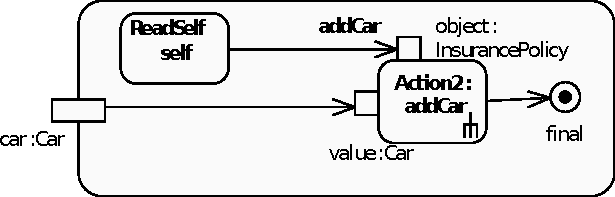
\includegraphics{images/addCar-activity_diagram}
\end{figure}

\begin{figure}
 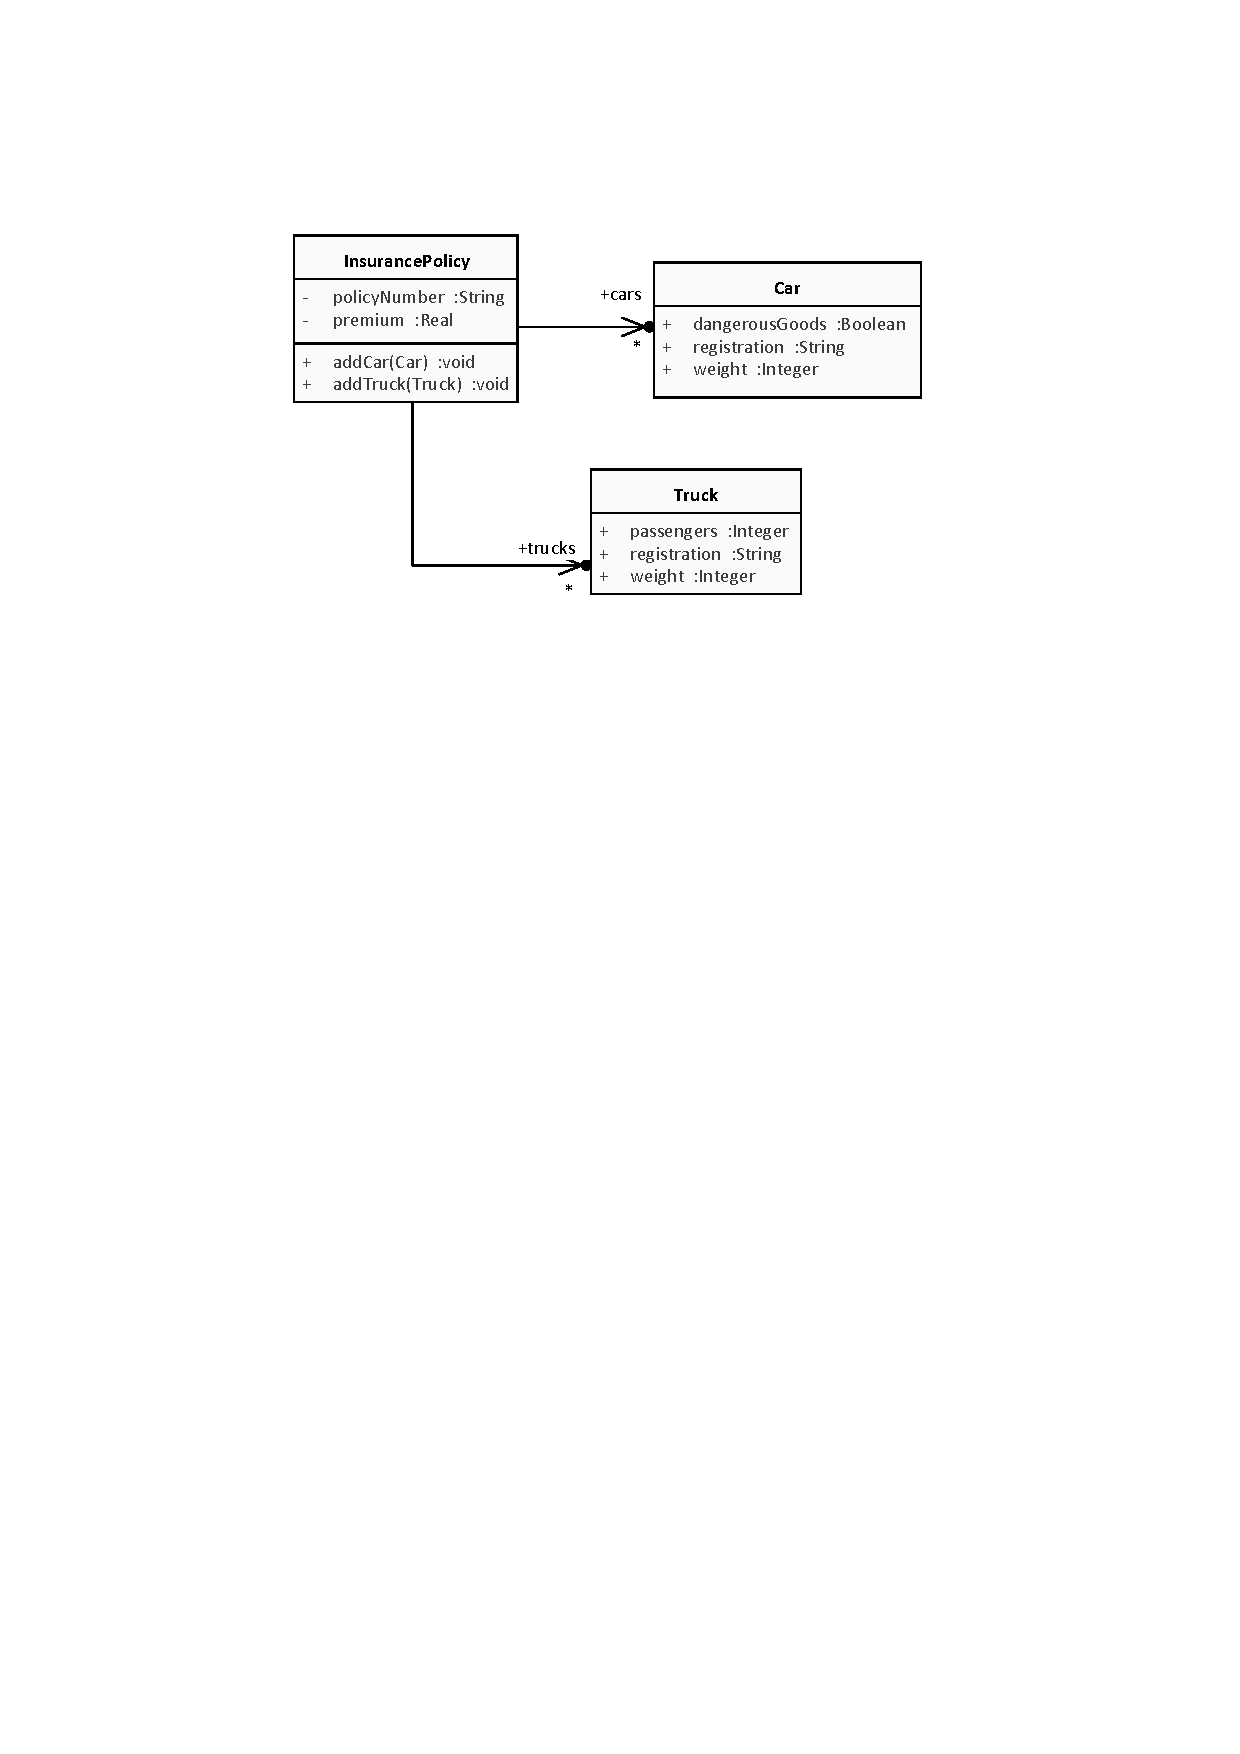
\includegraphics{images/addCar-class_diagram.pdf}
\end{figure}



\section{Tool chain and implementation}
For our tool chain we have relied on the moliz\footnote{source...} repository, mainly for the ability to execute the fUML models with
a virtual machine. The models are stored as XMI 
% usage of fUML reference implementation of BIG
% how to load models?
% how to execute models?
% how to apply queries and changes?

\subsection{Model refactoring}
Describe our tool chain, how we created models, how we load them, what information of the abstract syntax we use for refactoring, etc.

\subsection{GUI Integration}
Describe what we did with EMF.Refactor.

\section{Related Works}
% papers we read
% what we did that they didnt
We have compared our works with several other available papers. In [..] there is a discussion of uml refactings which covers ....

some related works such as ...

\section{Conclusion}
We conclude this paper with...

\bibliographystyle{acm}
\bibliography{references}

\end{document}
